% !TeX TXS-program:compile = txs:///xelatex/[--shell-escape]
% IACR Transactions CLASS DOCUMENTATION
% Written by Gaetan Leurent gaetan.leurent@inria.fr (2016-2018)
%
% To the extent possible under law, the author(s) have dedicated all
% copyright and related and neighboring rights to this software to the
% public domain worldwide. This software is distributed without any
% warranty.
%
% You should have received a copy of the CC0 Public Domain Dedication
% along with this software. If not, see
% <http://creativecommons.org/publicdomain/zero/1.0/>.

\documentclass[preprint]{iacrtrans}
\usepackage[utf8]{inputenc}

\setcounter{tocdepth}{4}

%% VERSION
\newcommand{\version}{v.1.0}


%% TITLE
\title{
  
\includegraphics[width=\columnwidth]{logo_zkEVM.png} \\ \vspace{0.3cm}
  Wiki Document\\ \vspace{0.3cm}
  Prover - eSTARK\\ \vspace{0.3cm}
  An Introduction to the Polygon zkEVM Proving Mechanism using \texttt{pil-stark} \\
  \version
}

\institute{}


\usepackage{caption}
\usepackage{subcaption}

% This package controls how hyperlinks are displayed
% https://es.overleaf.com/learn/latex/Hyperlinks
\usepackage{hyperref}
\hypersetup{colorlinks=true,linkcolor={red!80!black},urlcolor={blue!80!black}}

%Multiple columns
\usepackage{multicol}

% Used for super caligraphic font \mathscr{}
\usepackage{mathrsfs}

%This ensures spaces when using ensuremath and no $$ are used to introduce math
\usepackage{xspace}

%%%%%% BEGIN OF CODE HIGHLIGHTING ENVIRONMENTS %%%%%%

%   sudo apt install texlive-latex-extra
%   sudo apt install python-pip
%   pip install pygments
%   pip install pygments-lexer-babylon  #contains JSX
%   pip install pygments-lexer-solidity
%   pip install pygments pygments-lexer-babylon pygments-lexer-solidity


% *** COLOR COMMANDS ***
\definecolor{dblackcolor}{rgb}{0.0,0.0,0.0}
\definecolor{dbluecolor}{rgb}{0.01,0.02,0.5}
\definecolor{dgreencolor}{rgb}{0.2,0.4,0.0}
\definecolor{dgraycolor}{rgb}{0.30,0.3,0.30}
\newcommand{\dblue}{\color{dbluecolor}\bf}
\newcommand{\dred}{\color{dredcolor}\bf}
\newcommand{\dblack}{\color{dblackcolor}\bf}
\definecolor{light-gray}{gray}{0.96} %the shade of grey that stack exchange uses

\usepackage{showexpl}% already includes listings package
\makeatletter
\def\lst@filenamerpl{_\textunderscore $\textdollar}
\makeatother
\lstset{frame=shadowbox, basicstyle=\footnotesize\ttfamily, showstringspaces=false,
rulesepcolor=\color{black}, upquote=true}

\lstdefinestyle{scriptStyle}{
    basicstyle=\footnotesize,% control font of code
    preset=\footnotesize,% adjust font size of output
    numbers=none,
    frame=tlbr,
    pos=r,% want output on rightbackgroundcolor=\color{yellow!30},
    width=0.50\linewidth,
}

\lstdefinestyle{terms}{
    basicstyle=\scriptsize\ttfamily,% control font of code
    preset=\footnotesize,% adjust font size of output
}

\lstdefinestyle{termt}{
    basicstyle=\footnotesize\ttfamily,% control font of code
    preset=\footnotesize,% adjust font size of output
	numbers=none,
}

\lstdefinestyle{verb}{
    basicstyle=\footnotesize,% control font of code
    preset=\footnotesize,% adjust font size of output
    frame=tlbr,
    pos=r,% want output on right
%     backgroundcolor=\color{yellow!30},
    width=0.50\linewidth,
}

\lstdefinestyle{verbs}{
    basicstyle=\scriptsize,% control font of code
    preset=\scriptsize,% adjust font size of output
    frame=tlbr,
    pos=r,% want output on right
%     backgroundcolor=\color{yellow!30},
    width=0.50\linewidth,
}

\lstdefinestyle{verbt}{
    basicstyle=\tiny\ttfamily,% control font of code
    preset=\tiny\ttfamily,% adjust font size of output
    frame=tlbr,
    pos=r,% want output on right
%     backgroundcolor=\color{yellow!30},
    width=0.50\linewidth,
}

%Linter for circom
\usepackage{tcolorbox}
\tcbuselibrary{minted,skins,listings}
\definecolor{mybg}{rgb}{0.96,0.96,0.98}
% \lstset{
% 	backgroundcolor = \color{light-gray},
% 	showtabs = False,
% 	tabsize = 2,
% 	showspaces = False,
% 	showstringspaces = False,
% 	commentstyle = {\ttfamily\color{dgreencolor}},
% 	keywordstyle = {\ttfamily\color{dbluecolor}\bfseries},
% 	stringstyle = {\ttfamily\color{dgraycolor}\bfseries},
% 	language = circom,
% 	basicstyle = {\fontsize{7pt}{7pt}\ttfamily},
% 	aboveskip = 1em,
% 	belowskip = 1em,
% 	numbers = left,%none,
% 	numbersep=5pt,    %space line numbers from code
% 	xleftmargin=2em,
% 	frame=single,	% adds a frame around the code
% 	framexleftmargin=1.7em,
% 	numberstyle=\tiny,%\color{gray}
% 	emph = {proc,retp,endp,local},
% 	emphstyle = {\color{blue}\textbf},
% 	literate =
% 		{<==}{{{\color{dbluecolor}<==}}}2
% 		{==>}{{{\color{dbluecolor}==>{}}}}2
% 		{===}{{{\color{dbluecolor}==={}}}}2
% 		{<--}{{{\color{dbluecolor}<---{}}}}2
% 		{-->}{{{\color{dbluecolor}--->{}}}}2
% 		{*}{{{\color{dbluecolor}*{}}}}2
% }

\lstdefinelanguage{circom}{
	keywords=[1]{signal, input, output, public, <==, ==>, ===}, % generic keywords including crypto operations
  	keywordstyle=[1]\color{blue!70!}\bfseries,
	keywords=[3]{pragma, include},
  	keywordstyle=[3]\color{brown}\bfseries,
	keywords=[4]{for, if, var, else},
	keywordstyle=[4]\color{teal}\bfseries,
	keywords=[5]{template, component},
	keywordstyle=[5]\color{violet}\bfseries,
	identifierstyle=\color{black},
	sensitive=false,
	comment=[l]{//},
	morecomment=[s]{/*}{*/},
	commentstyle=\color{green!40!black}\ttfamily,
	stringstyle=\color{blue}\ttfamily,
%	morestring=[b]',
%	morestring=[b]"
}

\newtcblisting{circom}{
  listing engine=listings,
  colback=mybg,
  colframe=black!70,
  listing only,
  listing options={
    language={circom},
	basicstyle=\footnotesize\ttfamily,
    frame=none,
	numbers=none, %left
	numberstyle=\tiny,
	numbersep=9pt,
	tabsize=2,
	breaklines=true,
	showtabs=false,
	captionpos=b
  },
  left=0.2mm,
  top=0cm,
  bottom=0cm,
  boxrule=0.1mm
}

\newtcblisting{js}{
	listing engine=minted,
	colback=mybg,
	colframe=black!30,
	listing only,
	minted style=tango,
	minted language=js,
	minted options={linenos=false,texcl=true},
	left=0.2mm,
	top=0cm,
	bottom=0cm,
	boxrule=0.1mm
}

\lstdefinelanguage{Pil}{
	keywords=[1]{pol, commit, constant, in, is, connect, public, namespace}, % generic keywords including crypto operations
  keywordstyle=[1]\color{blue!70!}\bfseries,
	keywords=[3]{include}, % modules
  keywordstyle=[3]\color{brown}\bfseries,
	keywords=[4]{},% types; money and time units
	keywordstyle=[4]\color{teal}\bfseries,
	keywords=[5]{field, bool, u32, u16, u8},	% environment variables
	keywordstyle=[5]\color{violet}\bfseries,
	identifierstyle=\color{black},
	sensitive=false,
	comment=[l]{//},
	morecomment=[s]{/*}{*/},
	commentstyle=\color{green!40!black}\ttfamily,
	stringstyle=\color{blue}\ttfamily,
%	morestring=[b]',
%	morestring=[b]"
}

\newtcblisting{pil}{
  listing engine=listings,
  colback=mybg,
  colframe=black!70,
  listing only,
  listing options={
    language={Pil},
	basicstyle=\footnotesize\ttfamily,
    frame=none,
	numbers=none,
	numberstyle=\tiny,
	numbersep=9pt,
	tabsize=2,
	breaklines=true,
	showtabs=false,
	captionpos=b
  },
  left=0.2mm,
  top=0cm,
  bottom=0cm,
  boxrule=0.1mm
}

%%%%%%% END OF CODE HIGHLIGHTING ENVIRONMENTS %%%%%%%

\usepackage{url}
\usepackage{tikz}
\usepackage{graphicx} % Required for including images
\usepackage[font=small,labelfont=bf]{caption}  % Required for specifying captions to tables and figures


%%%%%%%%%%%%%%%%%%% BEGIN OF MACROS %%%%%%%%%%%%%%%%%%%

% Cryptocode: https://github.com/arnomi/cryptocode
\usepackage[
lambda,
operators,
landau, %este es el de bigO
probability,
%sets,
logic, %para or,and...
asymptotics,
keys
]{cryptocode}

% My own procedure blocks to show protocols
\createprocedureblock{mypb}{center, boxed}{}{}{linenumbering}
\createprocedureblock{mypbnonum}{center, boxed}{}{}{}

% Numbering style
\renewcommand{\pclnstyle}[1]{\text{#1}}
\renewcommand{\pclnseparator}{.}

% Hyphen inside mathmode
\mathchardef\mhyphen="2D

% Mathbb
\newcommand{\FF}{\ensuremath{\mathbb{F}}\xspace}
\newcommand{\KK}{\ensuremath{\mathbb{K}}\xspace}
\newcommand{\NN}{\ensuremath{\mathbb{N}}\xspace}
\newcommand{\ZZ}{\ensuremath{\mathbb{Z}}\xspace}

% Mathcal
\newcommand{\A}{\ensuremath{\mathcal{A}}\xspace}
\newcommand{\C}{\ensuremath{\mathcal{C}}\xspace}
\newcommand{\E}{\ensuremath{\mathcal{E}}\xspace}
\newcommand{\F}{\ensuremath{\mathcal{F}}\xspace}
\renewcommand{\H}{\ensuremath{\mathcal{H}}\xspace}
\newcommand{\I}{\ensuremath{\mathcal{I}}\xspace}
\renewcommand{\O}{\ensuremath{\mathcal{O}}\xspace}
\renewcommand{\P}{\ensuremath{\mathcal{P}}\xspace}
\newcommand{\R}{\ensuremath{\mathcal{R}}\xspace}
\renewcommand{\S}{\ensuremath{\mathcal{S}}\xspace}
\newcommand{\T}{\ensuremath{\mathcal{T}}\xspace}
\newcommand{\V}{\ensuremath{\mathcal{V}}\xspace}

% Mathscr
% \newcommand{\PPP}{\ensuremath{\mathscr{P}}\xspace}


% Mathfrak
\newcommand{\afr}{\ensuremath{\mathfrak{a}}\xspace}
\newcommand{\bfr}{\ensuremath{\mathfrak{b}}\xspace}

% Caligraphic Combiantions
\DeclareMathAlphabet{\mathpgoth}{OT1}{pgoth}{m}{n}
\newcommand{\plonk}{\ensuremath{\mathcal{P}\mathfrak{lon}\mathcal{K}}\xspace}
\newcommand{\plookup}{\ensuremath{\mathpgoth{plookup}}\xspace}

% Abbreviations
% \newcommand{\Pp}{\ensuremath{\mathcal{P}_{\textsf{poly}}\xspace}}
\newcommand{\MTR}{\ensuremath{\text{MTR}}\xspace}
\newcommand{\MTP}{\ensuremath{\text{MTP}}\xspace}
\newcommand{\LCC}{\ensuremath{\text{LCC}}\xspace}
\newcommand{\FRI}{\ensuremath{\textsf{F}}\xspace}
\newcommand{\z}{\ensuremath{\overline{z}}\xspace}
\newcommand{\fsel}{\ensuremath{f^{\text{sel}}}\xspace}
\newcommand{\tsel}{\ensuremath{t^{\text{sel}}}\xspace}
\newcommand{\Evals}{\ensuremath{\textsf{Evals}}\xspace}
\newcommand{\pparams}{\ensuremath{\text{pp}}\xspace}
\newcommand{\vparams}{\ensuremath{\text{vp}}\xspace}
\newcommand{\pre}{\ensuremath{\text{pre}}\xspace}
\newcommand{\tr}{\ensuremath{\text{tr}}\xspace}
\newcommand{\otr}{\ensuremath{\overline{\text{P}}}\xspace}
\newcommand{\im}{\ensuremath{\text{im}}\xspace}
\newcommand{\seed}{\ensuremath{\textsf{seed}}\xspace}
\newcommand{\transcript}{\ensuremath{\textsf{transcript}}\xspace}
\newcommand{\AIR}{\ensuremath{\textsf{A}}\xspace}
\newcommand{\eAIR}{\ensuremath{\textsf{eA}}\xspace}
\newcommand{\accept}{\ensuremath{\textsf{accept}}\xspace}
\newcommand{\reject}{\ensuremath{\textsf{reject}}\xspace}
\newcommand{\eFRI}{\ensuremath{\epsilon_{\textsf{FRI}}}\xspace}
\newcommand{\eSTARK}{\ensuremath{\epsilon_{\textsf{STARK}}}\xspace}
\newcommand{\eeSTARK}{\ensuremath{\epsilon_{\textsf{eSTARK}}}\xspace}
\newcommand{\eC}{\ensuremath{\epsilon_{\textsf{C}}}\xspace}
\newcommand{\ePlo}{\ensuremath{\epsilon_{\textsf{Plo}}}\xspace}
\newcommand{\eMulEq}{\ensuremath{\epsilon_{\textsf{MulEq}}}\xspace}
\newcommand{\eCon}{\ensuremath{\epsilon_{\textsf{Con}}}\xspace}
\newcommand{\eArgs}{\ensuremath{\epsilon_{\textsf{Args}}}\xspace}
\newcommand{\RS}{\ensuremath{\textsf{RS}[\FF,H,\rho]}\xspace}
\newcommand{\RSK}{\ensuremath{\textsf{RS}[\KK,H,\rho]}\xspace}
\newcommand{\LH}{\ensuremath{\textsf{LH}}\xspace}
\newcommand{\ID}{\ensuremath{\textsf{ID}}\xspace}

% C12
\newcommand{\POSEIDON}{\ensuremath{\texttt{POSEIDON12}}\xspace}
\newcommand{\acode}{\ensuremath{\texttt{a}}\xspace}
\newcommand{\CONST}{\ensuremath{\texttt{C}}\xspace}
\newcommand{\PARTIAL}{\ensuremath{\texttt{PARTIAL}}\xspace}
\newcommand{\CMULADD}{\ensuremath{\texttt{CMULADD}}\xspace}
\newcommand{\EVPOL}{\ensuremath{\texttt{EVPOL4}}\xspace}
\newcommand{\FFT}{\ensuremath{\texttt{FFT4}}\xspace}
\newcommand{\nextStep}{\ensuremath{\textsf{'}}\xspace}
\newcommand{\scale}{\ensuremath{\texttt{s}}\xspace}
\newcommand{\firstW}{\ensuremath{\texttt{firstW}}\xspace}
\newcommand{\firstWSquare}{\ensuremath{\texttt{firstW2}}\xspace}
\newcommand{\incW}{\ensuremath{\texttt{incW}}\xspace}
% Caligraphic Combiantions
 \DeclareMathAlphabet{\mathpgoth}{OT1}{pgoth}{m}{n}

% Abbreviations
\newcommand{\stoc}{\texttt{S2C}\xspace}
\newcommand{\ctos}{\texttt{C2S}\xspace}


% Make a nice emptyset
\let\oldemptyset\emptyset
\let\emptyset\varnothing

% Make a nice phi and epsilon
\let\oldphi\phi
\let\phi\varphi
\let\oldepsilon\epsilon
\let\epsilon\varepsilon

% Make a nice q.e.d. symbol
\renewcommand\qedsymbol{\ensuremath{\blacksquare}\xspace}

\theoremstyle{definition}
\newtheorem{protocol}{Protocol}
\newtheorem{bremark}{Remark}

\usepackage{paralist} % for compactitem environment

%%%%%%%%%%%%%%%%%%% END OF MACROS %%%%%%%%%%%%%%%%%%%

% \begin{pcvstack}[boxed, center]
% % \pcsetargs{codesize=\scriptsize{}}

% \procedure{}{
%   \textbf{Prover } \P(g_1(x))  \< \< \textbf{verifier } \V(g_1(x)) \\[][\hline]
%   \< \sendmessageright{top={$f_1(s)$, $f_2(s)$}} \< \\[-2mm]
%   \< \sendmessageleft{top={randomness}} \< \\[-2mm]
%   \< \sendmessageright{top={$f_3(s)$}} \< \\[-2mm]
%   \< \< \text{Samples a random } z \in \FF \text{ and computes } z\vec{g}. \\[-2mm]
%   \< \sendmessageleft{top={$z$}} \< \\[-2mm]
%   \text{Computes evaluations:} \< \< \\
%   \t g_1(z), f_1(z), f_2(z), f_3(z) \< \< \\[-2mm]
%   \< \sendmessageright{top={$g_1(z)$, $f_1(z)$, $f_2(z)$, $f_3(z)$}} \< \\[-2mm]
%   \< \sendmessageleft{top={$v$}} \< \\[-2mm]
%   \< \sendmessageright{top={$\pi$}} \< \\[-2mm]
%   \< \< \text{Verifies the opening proof } \pi \text{ and checks that:} \\
%   \< \< \t g_1(z)(f_1(z) + f_2(z)) - f_3(z) = 0
% }
% \end{pcvstack}

\newcommand{\definedir}[2]{\newcommand{#1}{#2}}
\definedir{\starkintrodir}{..}


\begin{document}
\begin{titlepage}
\centering
\maketitle
\today
\end{titlepage}

% use optional argument because the \LaTeX command breaks the PDF keywords
% \keywords[\publname, ToSC, TCHES, LaTeX]{TBD \and TBD}

%{\hypersetup{linkcolor=.}\tableofcontents}

\newpage
% !TeX spellcheck = en_GB
% !TeX TXS-program:compile = txs:///xelatex/[--shell-escape]
% !TeX root = ../build/estark.tex


The setting for STARK proofs are machine-like computations from which we can derive a certain arithmetization, giving us a set of constraints describing its correct execution. The polynomial interpolating the constrained values that arise from a certain arithmetization can, in fact, depend on the inputs of the computation itself giving what we call \textbf{committed polynomials} and, by definition, should be computed once per proof. However, a polynomial that is completely independent of the input values so it is kept constant among several executions of the same computation should be computed only once per arithmetization. The former kind of polynomials are called \textbf{constant polynomials} and, together with the constraints, represent the computation that is being executed, so that they are publicly available for both the prover and the verifier, unlike the committed ones, which are not directly available to the verifier.

\begin{figure}[H]
\centering
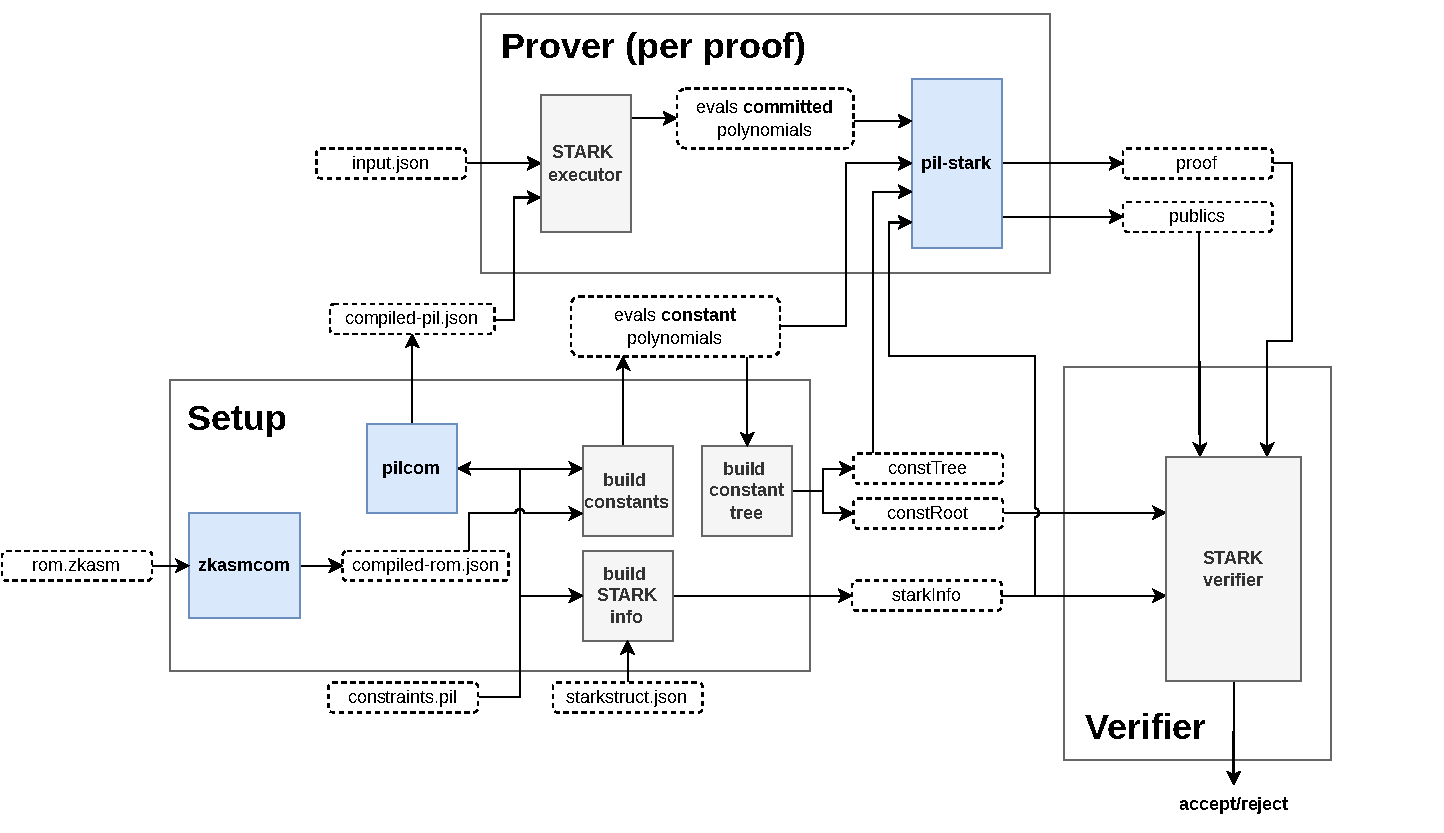
\includegraphics[width=0.9\columnwidth]{\zkevmdir/figures/estark/proving-scheme.drawio.pdf}
\caption{Proving Architecture Scheme in zkEVM.}
\label{fig:proving-arch-scheme}
\end{figure}

Due to the fact that all the constant polynomials do not depend on the particular inputs of a certain computation, we can split the processes that make up the generation of a proof in two: the \textit{setup phase} and the \textit{proving phase}. This allows to execute both processes separately, which is highly important in order not to execute the constants' computation per proof, drastically increasing the proving time.

\paragraph*{The Setup Phase}

The \textit{setup phase} performs all the pre-processing. The setup is only done once per state machine definition, allowing to reuse it whether the definition does not change. The definition of a machine-like computation with \texttt{pil-stark} has three parts:

\begin{itemize}

\item \textbf{The program:} A \texttt{rom.json} file to build the computation.  This file serves as the ``guide" for constructing the computation, detailing the specific steps and operations that define the logic of the state machine. In the zkEVM, this file is obtained by compiling (using the \texttt{zkasmcom} compiler) a \texttt{.zkasm} file wrote in zkASM language, an assembly language specific for the zkEVM.

\item \textbf{The constraints:} The PIL description of the STARK state machine, that is to say, the constraints that define the correctness of the execution trace. In the zkEVM, the constraints are wrote into a \texttt{.pil} file using PIL, standing for Polynomial Identity Language. The \texttt{pilcom} parser is written with \url{https://github.com/zaach/jison}, which generates bottom-up parsers in JavaScript. This compiled constraints file will be used by the prover to compute all the polynomials involved in the proving procedure.

\item \textbf{The configuration:} The configuration of the FRI used in the STARK proof, inside a \texttt{starkStruct} file, specifying, among other, the blowup factor, the size of the trace and its LDE (Low Degree Extension), the number of queries to be performed and the willing-to-use step configuration.

\end{itemize}

Let's delve into each block service within the setup zone of the Figure \ref{fig:proving-arch-scheme}.

\begin{itemize}

\item \textbf{Build Constants}: This service is in charge of generating a binary for the constant polynomials' evaluations from a given compiled program \texttt{rom.json} and a set of constraints \texttt{file.pil}. The compiled program is directly used to accurately populate the polynomial values based on the its rules, while the PIL file is only used to extract the polynomial degree, also known as the length of the execution trace. This service is run using the script \texttt{main\_buildconstants} from the \href{https://github.com/0xPolygonHermez/zkevm-proverjs}{\texttt{zkevm-proverjs}} repository.

\item \textbf{Build Stark Info}: This block, managed by the \texttt{main\_genstarkinfo} script, plays a pivotal role in the setup phase. This service involves the generation of a \texttt{starkInfo} file, containing essential information required for the STARK proof generation process. Beyond the conventional \texttt{starkStruct} details, this file incorporates additional information intrinsic to the eSTARK protocol. Notably, it integrates expressions computation helpers tailored for the polynomials constructed in each of the eSTARK phases, which will be explained later on.

\item \textbf{Build Constant Tree}: Executed through the \texttt{main\_buildconsttree} script, is tasked with the creation of a structured representation of constant polynomials. This tree-like structure facilitates efficient manipulation and retrieval of constant polynomial values during the proof generation process. It also generates the Merkle root of its corresponding tree for the verifier, which we call constant root (\texttt{constRoot}).

\end{itemize}

\paragraph*{The Proving Phase}

In the \textit{proving phase}, the Prover executes all the processes that, given an input, generate a proof for the computation. The STARK executor process computes the evaluations of the polynomials that are going to be committed. To do so, it takes the names and descriptions of the polynomials from the parsed PIL and the provided inputs. Observe that, since the values of the committed polynomials are strongly dependent on the inputs, this procedure should be executed once per proof, unlike the setup phase.

Finally, the \texttt{pil-stark} \textsf{eSTARK} prover process takes the evaluations of both the constant and the committed polynomials of the previous steps and all the information stored in the \texttt{starkInfo} object in order to generate the corresponding \textsf{eSTARK} proof and the associated public values for which the proof is valid. We use the \textsf{eSTARK} protocol, which is specially designed to proof PIL statements. A complete description of the \texttt{eSTARK} protocol can be found in \cite{EPRINT:MGBT}.

As a summary, the \textsf{eSTARK} protocol is composed on two main stages:

\begin{itemize}
\item \textit{Low-Degree Reduction phase}: Following \cite{EPRINT:StarkWare21}, first of all, we obtain a polynomial called FRI which codifies the validity of the values of the trace according to the PIL into the fact that it has low degree. This polynomial is committed to the verifier, as well as several previous polynomials that are used to provide consistency checks between them.  This phase, however, differs from the one described in \cite{EPRINT:StarkWare21} because PIL also accepts, apart from polynomial equalities, arguments such lookups, permutations or even copy-constraints (called connection arguments). Hence, this phase needs to be adapted in order to proof the correctness of each of the enumerated arguments. This serves as a motivation to call this protocol \textsf{eSTARK}, standing for \textit{extended STARK}.

\item \textit{FRI phase}: After obtaining the so called FRI polynomial, the prover and the verifier are involved into a FRI Protocol, aiming for proving that the committed polynomial has low degree (more concretely, it proves that the committed values of the polynomials raise a function that is close enough to a polynomial of low degree.

\end{itemize}

The first stage can, in turn, be divided into several rounds. Below, we describe in a high level what is each of the rounds aiming.

\begin{itemize}

\item \textit{Round 1:} Given the trace column polynomials interpolating the execution trace, the prover commits to them.

\item \textit{Round 2:} The prover commits, for each lookup argument, to the $h$-polynomials of the modified \plookup version described in \cite{EPRINT:PFMBM22} (see \cite{EPRINT:GabWil20} for more information about \plookup protocol).

\item \textit{Round 3:} The prover commits to the grand-product polynomials for each of the arguments appearing in the PIL together with some intermediate polynomials used to reduce the degree of the grand products. This is due to the fact that \texttt{pil-stark} imposes a degree bound when committing to a polynomial. See \cite{EPRINT:GabWilCio19, EPRINT:GabWil20} for the specification of the grand-products of each of the different arguments allowed in PIL.

\item \textit{Round 4:} The prover commits to the $2$ polynomials $Q_1, Q_2$ arising from the splitting of the quotient polynomial $Q$ described in the \texttt{eSTARK} protocol.

\item \textit{Round 5:} The prover provides the verifier with all the necessary evaluations of the polynomials so that he/she can execute the corresponding checks.

\item \textit{Round 6:} The prover receives two randomness from the verifier which are used to construct the previously described FRI polynomial. Then, the prover and the verifier are involved into a FRI Protocol, ending with the prover sending the corresponding FRI proof to the verifier.

\end{itemize}


The \href{https://github.com/0xPolygonHermez/pil-stark}{\texttt{pil-stark}} package provides an implementation of a \textbf{Prover} instance at the \texttt{main\_prover.js} script.


\paragraph*{Verification Phase}

After the generation of the proof, it is sent to the designated \textbf{Verifier} instance. The \textbf{Verifier} is in charge of executing a well-defined procedures stating the correctness of the proof submitted by the \textbf{Prover}. This correctness, in turn, signifies the cryptographic correctness of the initial computational statement. The \href{https://github.com/0xPolygonHermez/pil-stark}{\texttt{pil-stark}} package provides an implementation of a \textbf{Verifier} instance at the \texttt{main\_verifier.js} script.

\newpage
\bibliographystyle{alpha}
\bibliography{../bib/bibliography}

\newpage
\appendix

\end{document}